\chapter{Web Application}

This chapter presents a simple Flask application connecting to the Oracle database. 
It employs multiple routes for the main operations:

\begin{itemize}
    \item \textbf{Order management.} Users can insert new orders (\texttt{/add\_order}) 
    and assign them to teams (\texttt{/assign\_order}).
    \item \textbf{Customer registration.} A new customer can be added (\texttt{/register\_customer}), 
    supporting both ''individual'' and ''business'' types.
    \item \textbf{Team statistics.} Routes like \texttt{/team\_stats} and \texttt{/teams\_list} 
    give information about total orders handled by a specific team, the total cost of the orders handled by a specific team and information about performance score of all teams.
\end{itemize}

The application follows this directory structure:
\begin{verbatim}
webapp/
├── database.py
├── app.py
├── static/        
│   └── css/
│       └── style.css
└── templates/      
    ├── base.html
    ├── home.html
    ├── add_order.html
    ├── assign_order.html
    ├── register_customer.html
    ├── team_stats.html
    └── teams_list.html
\end{verbatim}

The code centralizes database access in a separate \texttt{database.py} module. In production this file will be replaced placing the database credentials in an \texttt{env}, accessed with the library \texttt{python-dotenv}. 

Procedure and function calls (e.g., \texttt{registerCustomer}, \texttt{addOrder}, or \texttt{assignOrderToTeam}) are used to interact with the Oracle schema, ensuring logic remains in the PL/SQL layer.

\begin{figure}[H]
    \centering
    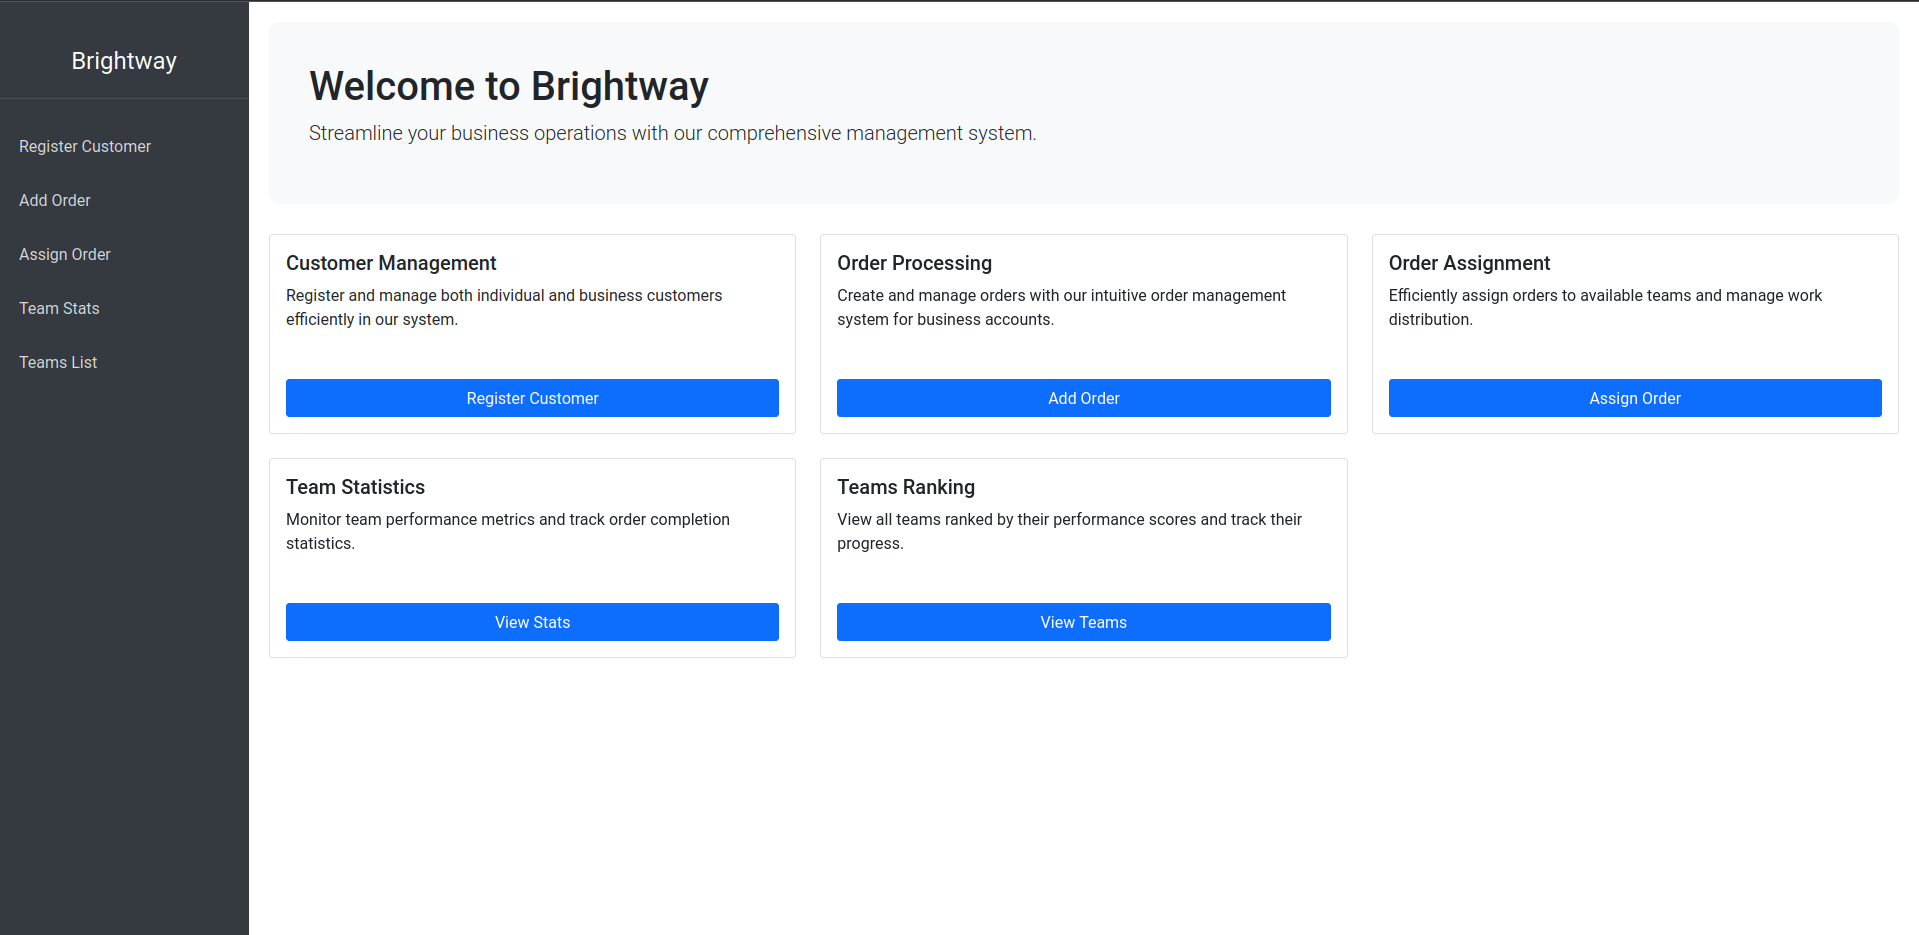
\includegraphics[width=0.8\textwidth]{img/web_app/home.png}
    \caption{Home page of the web application.}
\end{figure}

\begin{figure}[H]
    \centering
    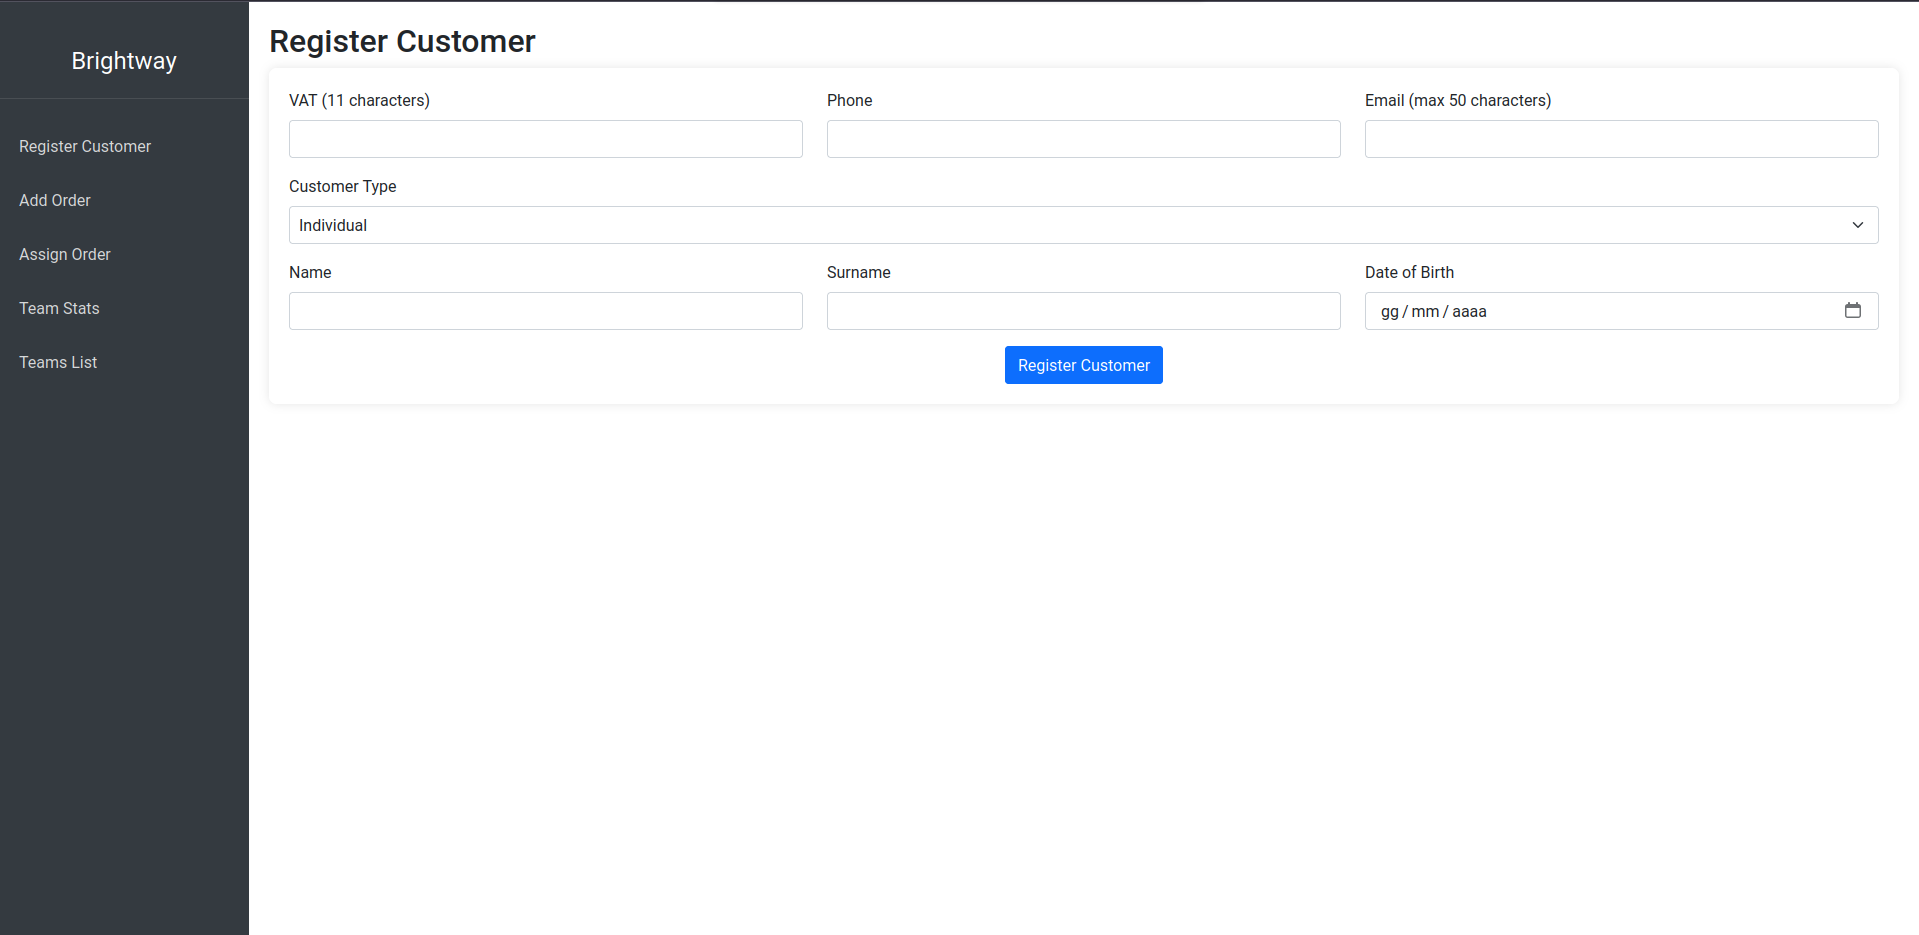
\includegraphics[width=0.8\textwidth]{img/web_app/customer_i.png}
    \caption{Customer registration form for individual customers.}
\end{figure}

\begin{figure}[H]
    \centering
    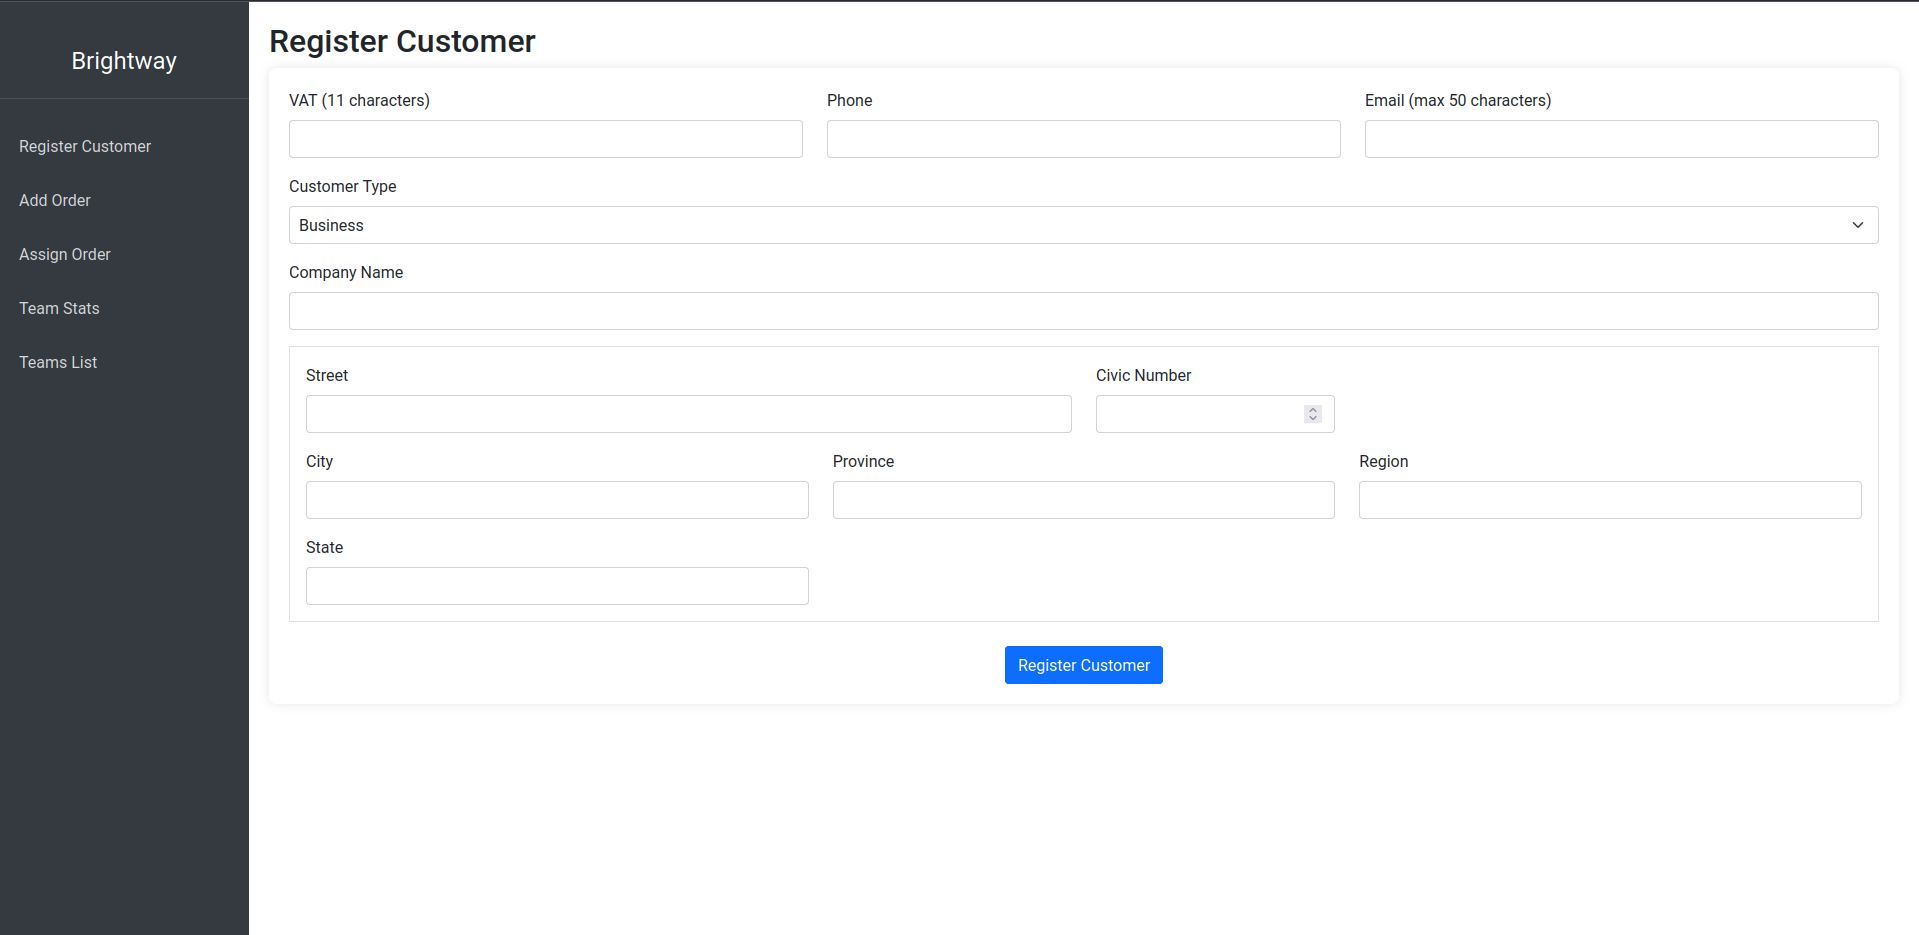
\includegraphics[width=0.8\textwidth]{img/web_app/customer_b.png}
    \caption{Customer registration form for business customers.}
\end{figure}

\begin{figure}[H]
    \centering
    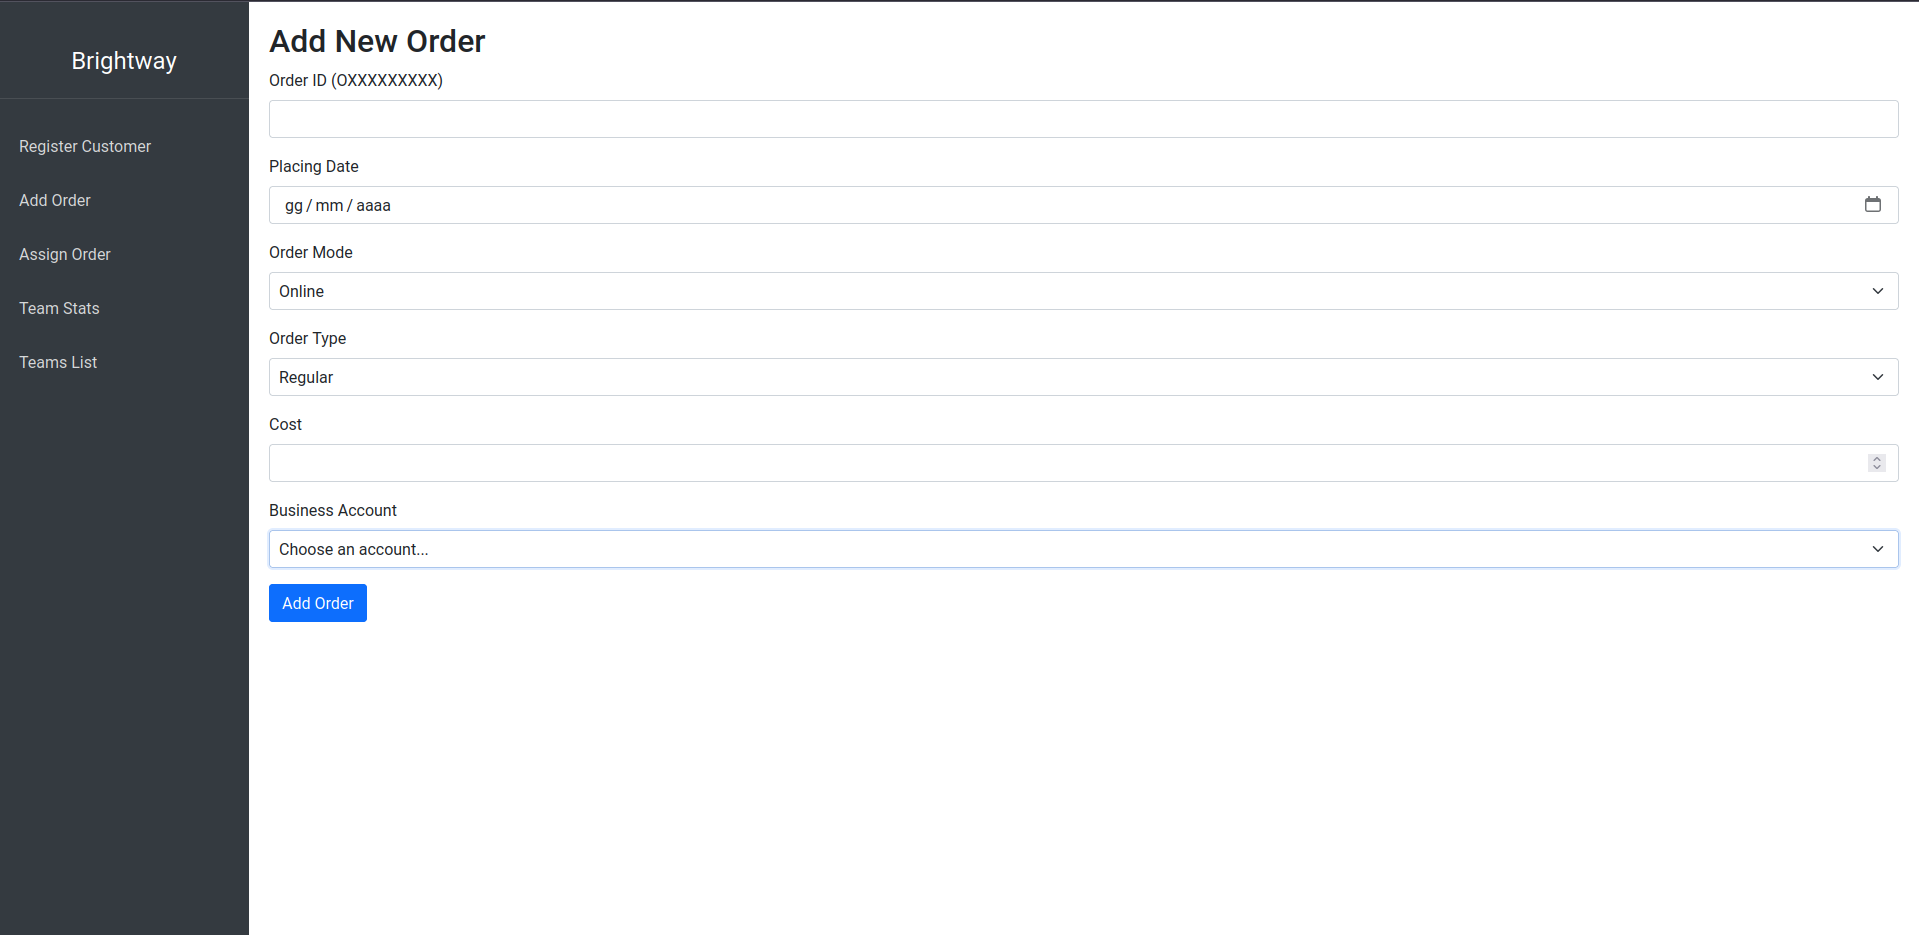
\includegraphics[width=0.8\textwidth]{img/web_app/add.png}
    \caption{Order insertion form.}
\end{figure}

\begin{figure}[H]
    \centering
    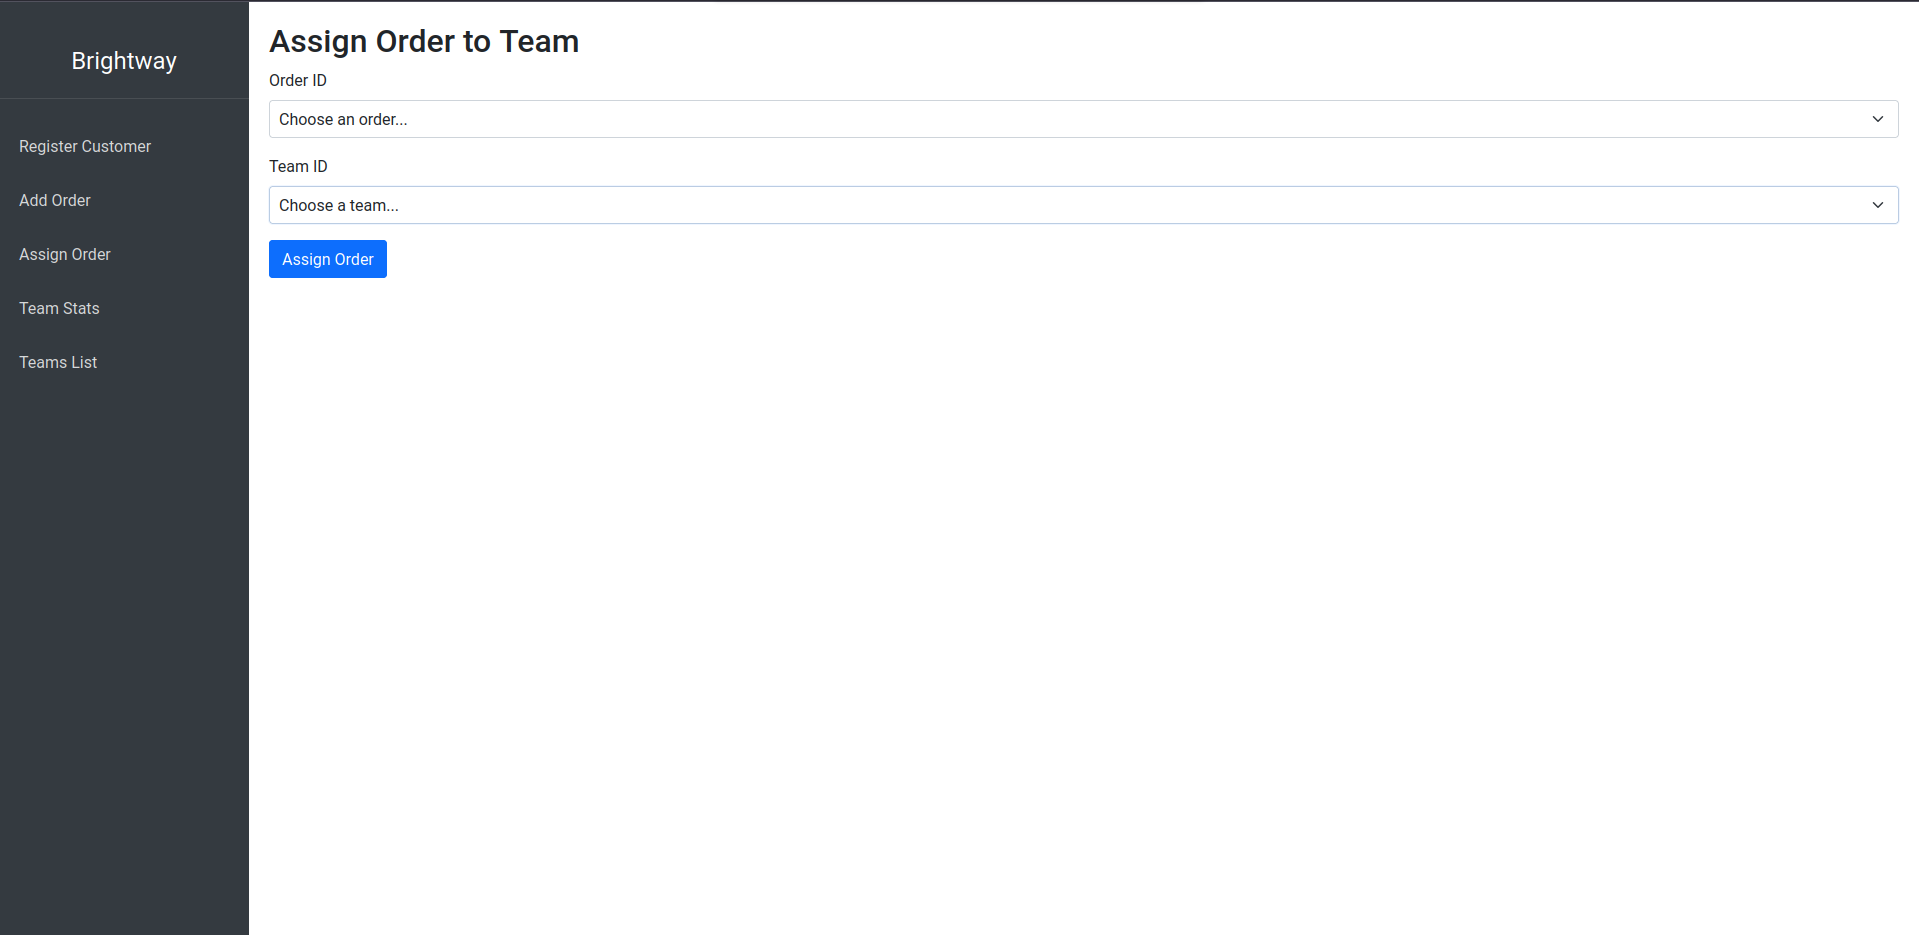
\includegraphics[width=0.8\textwidth]{img/web_app/assign.png}
    \caption{Order assignment form.}
\end{figure}

\begin{figure}[H]
    \centering
    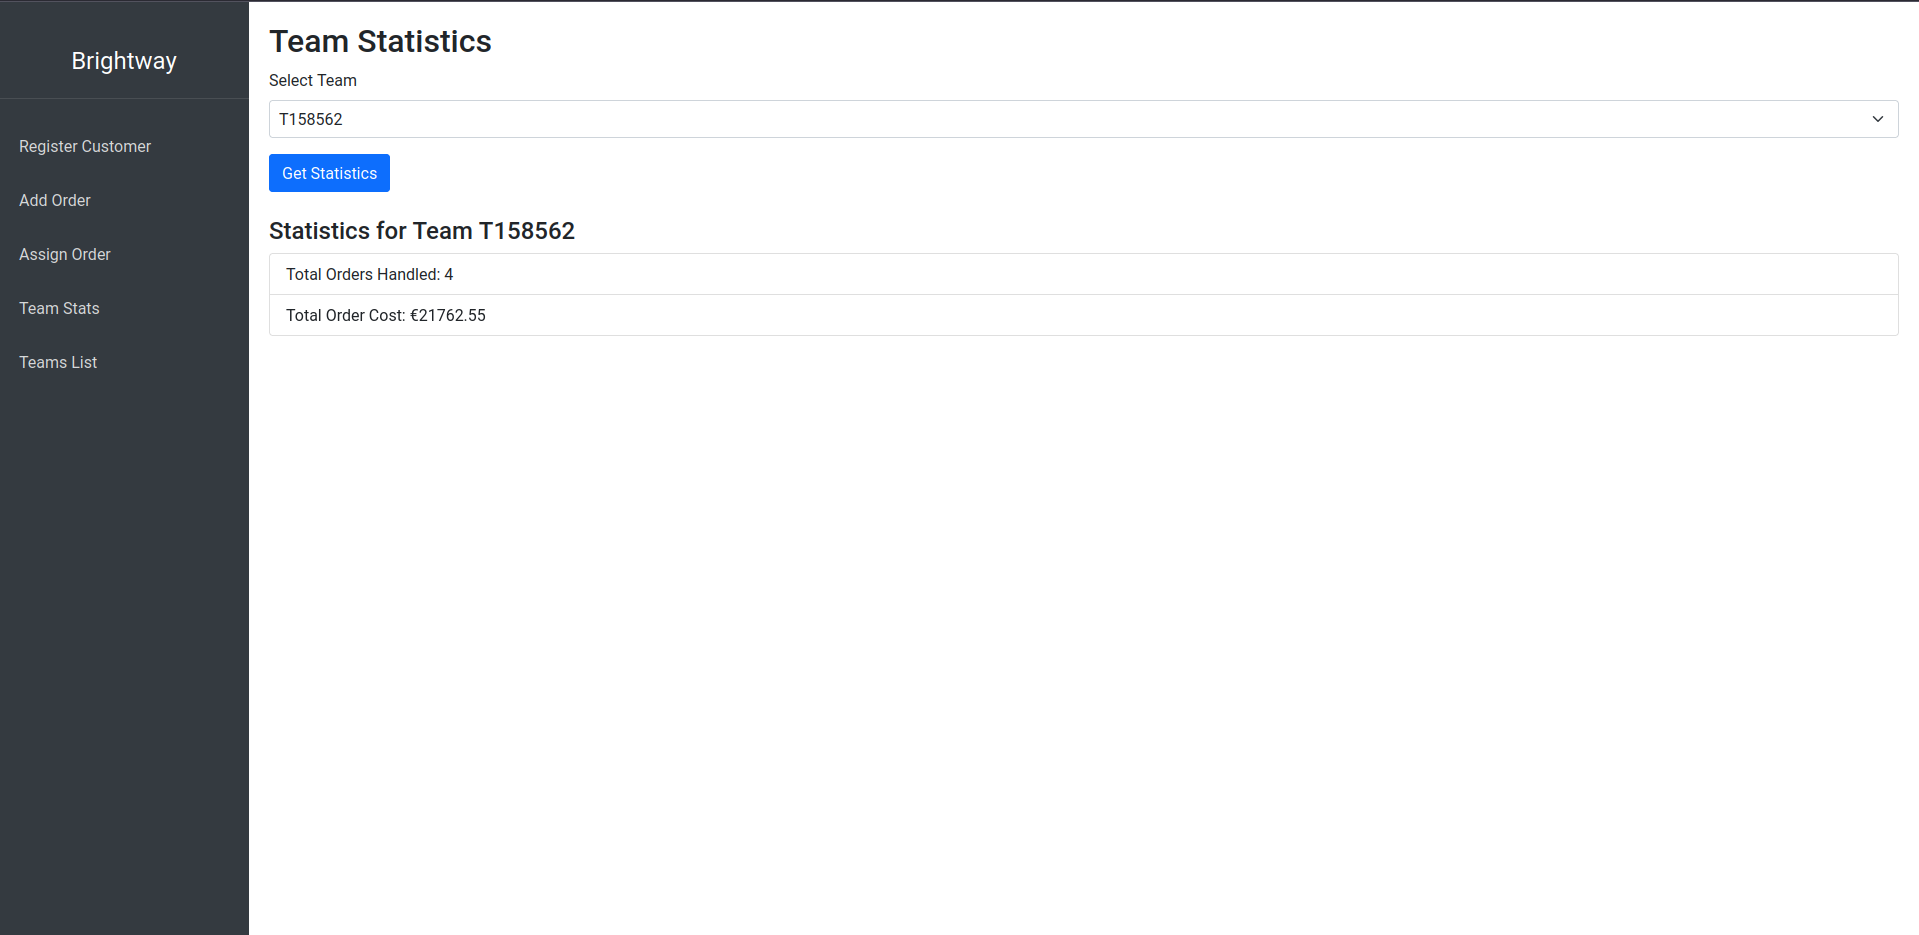
\includegraphics[width=0.8\textwidth]{img/web_app/stats.png}
    \caption{Team statistics page.}
\end{figure}

\begin{figure}[H]
    \centering
    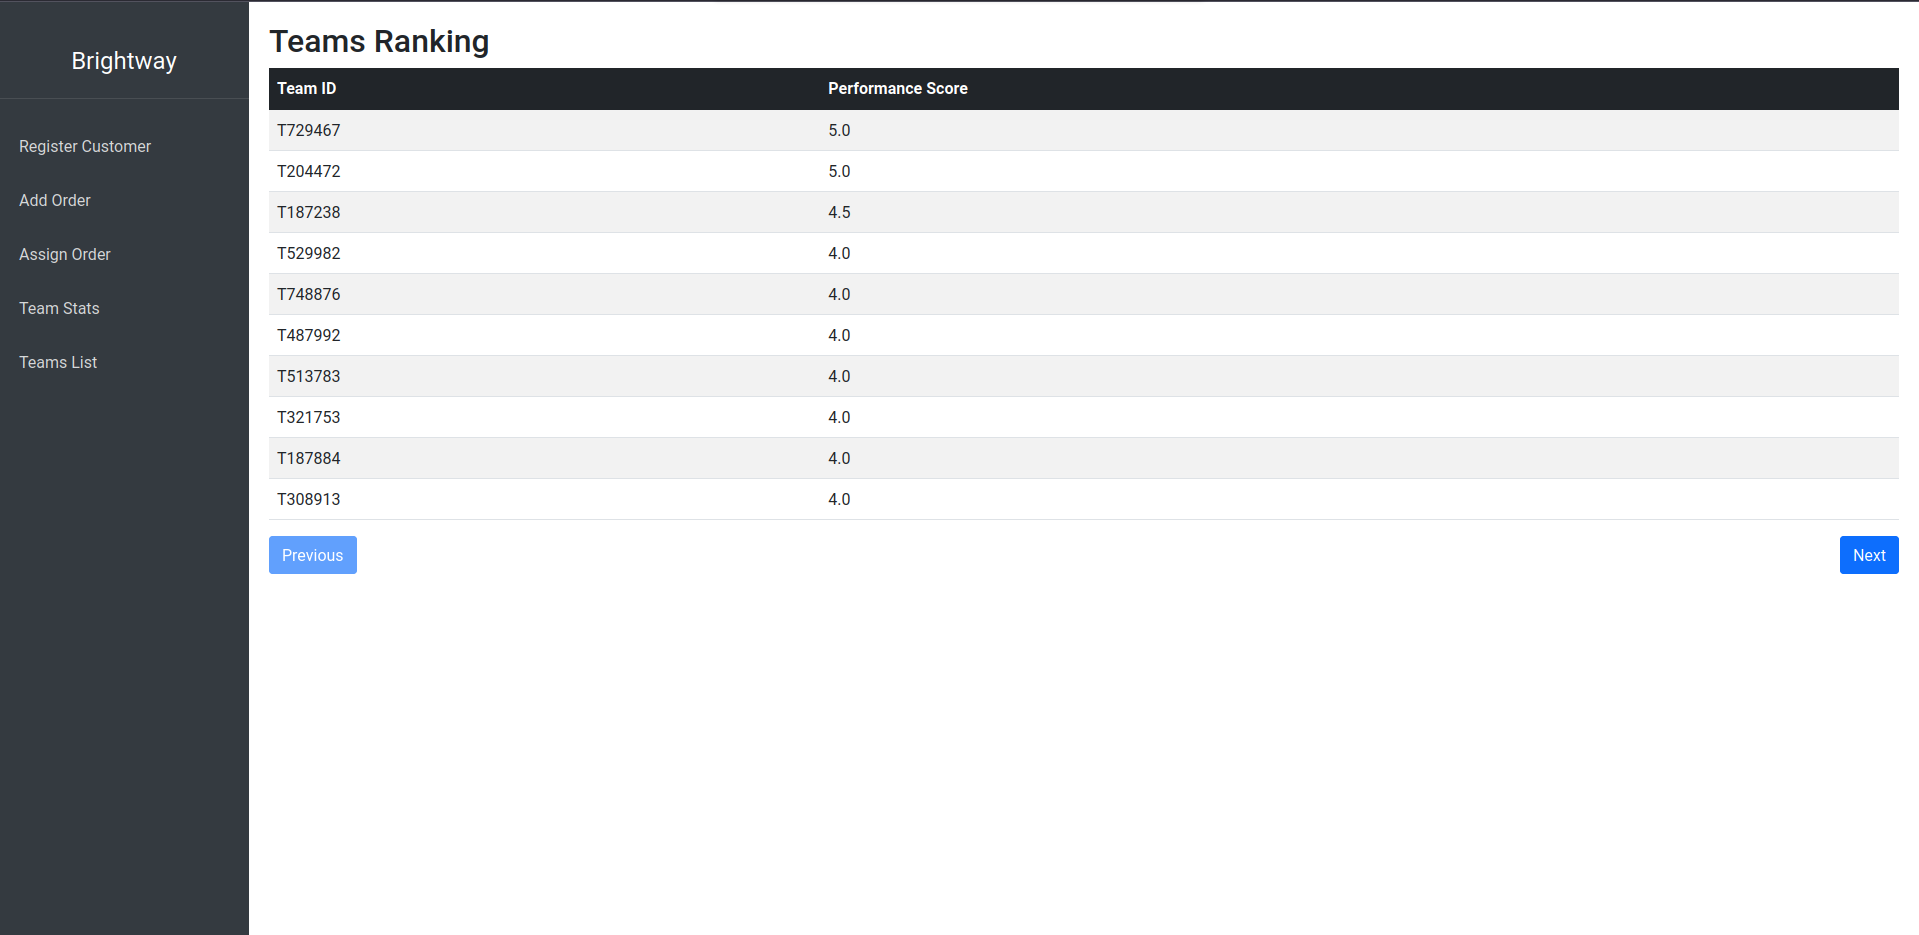
\includegraphics[width=0.8\textwidth]{img/web_app/list.png}
    \caption{List of teams sorted by performance score.}
\end{figure}

Here we present only the code of \texttt{app.py} for brevity:

\begin{lstlisting}[language=python]
from flask import Flask, render_template, request, redirect, url_for
from datetime import datetime
import database
import oracledb

app = Flask(__name__)

@app.route('/')
def index():
    return render_template('base.html')

# Op (1)
@app.route('/register_customer', methods=['GET', 'POST'])
def register_customer():
    if request.method == 'POST':
        try:
            conn = database.get_connection()
            cursor = conn.cursor()
            
            vat = request.form['vat']
            phone = request.form['phone']
            email = request.form['email']
            cust_type = request.form['type']
            
            # Always create an AddressTY object (even if empty for individual)
            address_type = conn.gettype('ADDRESSTY')
            address_obj = address_type.newobject()
            address_obj.STREET = None
            address_obj.CIVICNUM = None
            address_obj.CITY = None
            address_obj.PROVINCE = None
            address_obj.REGION = None
            address_obj.STATE = None

            if cust_type == 'individual':
                name = request.form['name']
                surname = request.form['surname']
                dob = datetime.strptime(request.form['dob'], '%Y-%m-%d').date()
                company_name = None
            else:
                name = None
                surname = None
                dob = None
                company_name = request.form['companyName']
                address_obj.STREET = request.form['street']
                address_obj.CIVICNUM = int(request.form['civicNum'])
                address_obj.CITY = request.form['city']
                address_obj.PROVINCE = request.form['province']
                address_obj.REGION = request.form['region']
                address_obj.STATE = request.form['state']

            cursor.callproc('registerCustomer', [
                vat, phone, email, cust_type,
                name, surname, dob,
                company_name, address_obj
            ])
                    
            conn.commit()
            cursor.execute("""
                SELECT CODE 
                FROM BusinessAccountTB b 
                WHERE b.customer.VAT = :vat
            """, [vat])
            result = cursor.fetchone()
            if result:
                return render_template('register_customer.html', business_account=result[0])
            return render_template('register_customer.html')
            
        except oracledb.DatabaseError as e:
            error, = e.args
            return render_template('register_customer.html', error=error.message)
        finally:
            cursor.close()
            conn.close()
    
    return render_template('register_customer.html')

# Op. (2)
@app.route('/add_order', methods=['GET', 'POST'])
def add_order():
    if request.method == 'POST':
        try:
            conn = database.get_connection()
            cursor = conn.cursor()
            
            # Form data
            order_id = request.form['order_id']
            placing_date = datetime.strptime(request.form['placing_date'], '%Y-%m-%d').date()

            guid = False            
            if order_id == "":
                # execute sys_guid() to get a unique identifier 
                cursor.execute("SELECT RAWTOHEX(SYS_GUID()) FROM dual")
                order_id = cursor.fetchone()[0]
                guid = True
            
            cursor.callproc('addOrder', [
                order_id,
                placing_date,
                request.form['order_mode'],
                request.form['order_type'],
                float(request.form['cost']),
                request.form['business_account']
            ])
            
            conn.commit()
            # Get business accounts before rendering template
            cursor.execute("SELECT CODE FROM BusinessAccountTB")
            business_accounts = [row[0] for row in cursor.fetchall()]
            if guid:
                return render_template('add_order.html', success="Order added successfully! Order ID: " + order_id, business_accounts=business_accounts)
            return render_template('add_order.html', success="Order added successfully!", business_accounts=business_accounts)
            
        except oracledb.DatabaseError as e:
            error, = e.args
            # Get business accounts even when there's an error
            cursor.execute("SELECT CODE FROM BusinessAccountTB")
            business_accounts = [row[0] for row in cursor.fetchall()]
            return render_template('add_order.html', error=error.message, business_accounts=business_accounts)
        finally:
            cursor.close()
            conn.close()
    
    # Handle GET request
    try:
        conn = database.get_connection()
        cursor = conn.cursor()
        cursor.execute("SELECT CODE FROM BusinessAccountTB")
        business_accounts = [row[0] for row in cursor.fetchall()]
        return render_template('add_order.html', business_accounts=business_accounts)
    except oracledb.DatabaseError as e:
        error, = e.args
        return render_template('add_order.html', error=error.message)
    finally:
        if 'cursor' in locals():
            cursor.close()
        if 'conn' in locals():
            conn.close()
    

# Op. (3)
@app.route('/assign_order', methods=['GET', 'POST'])
def assign_order():
    if request.method == 'POST':
        try:
            conn = database.get_connection()
            cursor = conn.cursor()
            cursor.callproc('assignOrderToTeam', [
                request.form['order_id'],
                request.form['team_id']
            ])
            conn.commit()
            # Get lists for dropdowns
            cursor.execute("SELECT ID FROM OrderTB WHERE team IS NULL")
            orders = [row[0] for row in cursor.fetchall()]
            cursor.execute("SELECT ID FROM TeamTB")
            teams = [row[0] for row in cursor.fetchall()]
            return render_template('assign_order.html', orders=orders, teams=teams, success="Order assigned successfully!")
        except oracledb.DatabaseError as e:
            error, = e.args
            # Get lists for dropdowns even when there's an error
            cursor.execute("SELECT ID FROM OrderTB WHERE team IS NULL")
            orders = [row[0] for row in cursor.fetchall()]
            cursor.execute("SELECT ID FROM TeamTB")
            teams = [row[0] for row in cursor.fetchall()]
            return render_template('assign_order.html', error=error.message, orders=orders, teams=teams)
        finally:
            cursor.close()
            conn.close()

    # Get lists for dropdowns
    try:
        conn = database.get_connection()
        cursor = conn.cursor()
        # Get unassigned orders
        cursor.execute("SELECT ID FROM OrderTB WHERE team IS NULL")
        orders = [row[0] for row in cursor.fetchall()]
        # Get all teams
        cursor.execute("SELECT ID FROM TeamTB")
        teams = [row[0] for row in cursor.fetchall()]
        return render_template('assign_order.html', orders=orders, teams=teams)
    except oracledb.DatabaseError as e:
        error, = e.args
        return render_template('assign_order.html', error=error.message)
    finally:
        cursor.close()
        conn.close()

# Op. (4A), (4B)
@app.route('/team_stats', methods=['GET', 'POST'])
def team_stats():
    if request.method == 'POST':
        team_id = request.form['team_id']
        try:
            conn = database.get_connection()
            cursor = conn.cursor()
            
            # Get total orders
            cursor.execute("SELECT totalNumOrder(:1) FROM DUAL", [team_id])
            total_orders = cursor.fetchone()[0]
            
            # Get total cost
            cursor.execute("SELECT totalOrderCost(:1) FROM DUAL", [team_id])
            total_cost = cursor.fetchone()[0]
            
            # Get teams for dropdown
            cursor.execute("SELECT ID FROM TeamTB")
            teams = [row[0] for row in cursor.fetchall()]
            
            return render_template('team_stats.html', 
                                 total_orders=total_orders,
                                 total_cost=total_cost,
                                 team_id=team_id,
                                 teams=teams)
        except oracledb.DatabaseError as e:
            error, = e.args
            return render_template('team_stats.html', error=error.message)
        finally:
            cursor.close()
            conn.close()
    
    # For GET request, just get teams for dropdown
    try:
        conn = database.get_connection()
        cursor = conn.cursor()
        cursor.execute("SELECT ID FROM TeamTB")
        teams = [row[0] for row in cursor.fetchall()]
        return render_template('team_stats.html', teams=teams)
    except oracledb.DatabaseError as e:
        error, = e.args
        return render_template('team_stats.html', error=error.message)
    finally:
        if 'cursor' in locals():
            cursor.close()
        if 'conn' in locals():
            conn.close()

# Op. (5)
@app.route('/teams_list', methods=['GET', 'POST'])
def teams_list():
    # Default number of rows to display
    rows_to_display = 10
    # Get the current offset from query parameters, default to 0
    offset = int(request.args.get('offset', 0))
    
    if offset < 0:
        offset = 0
    
    if request.method == 'POST':
        # Get number of rows from form input
        rows_to_display = int(request.form.get('num_rows', 20))
        # Reset offset when form is submitted
        offset = 0

    try:
        conn = database.get_connection()
        cursor = conn.cursor()
        
        # Get total count of teams
        cursor.execute("SELECT COUNT(*) FROM TeamTB")
        total_teams = cursor.fetchone()[0]
        
        # Modified query to include OFFSET
        cursor.execute("""
            SELECT ID, performanceScore 
            FROM TeamTB 
            ORDER BY performanceScore DESC
            OFFSET :1 ROWS FETCH NEXT :2 ROWS ONLY
        """, [offset, rows_to_display])
        teams = cursor.fetchall()
        
        # Check if there are more teams to show
        has_next = (offset + rows_to_display) < total_teams
        
        return render_template('teams_list.html',
                               teams=teams,
                               num_rows=rows_to_display,
                               offset=offset,
                               has_next=has_next)
    except oracledb.DatabaseError as e:
        error, = e.args
        return render_template('teams_list.html', error=error.message)
    finally:
        cursor.close()
        conn.close()

if __name__ == '__main__':
    app.run(debug=True)
\end{lstlisting}